\documentclass[a4paper]{article}%字号5号
\usepackage{xpatch}
\ExplSyntaxOn
\makeatletter
\xpatchcmd{\@maketitle}
{
    \@title
}
{
    \heiti\zihao{3}\@title
}
{}{\fail}
\xpatchcmd{\@maketitle}
{
    \@author
}
{
    \kaishu\zihao{-4}\@author
}
{}{\fail}
\makeatother
\ExplSyntaxOff
\usepackage{ctex}%输出汉字
\usepackage{times}%英文字体
\title{主定理(Master Theorem)}%黑体三号,行距1.5倍
\author{范潇\phantom{1}吴靖阳\phantom{1}陈思同}%小四字号,1.5倍行距,仿宋
\date{}%去除日期
\linespread{1.5}%行间距1.5倍
\usepackage{amsmath,amsthm,amssymb,graphicx}
\usepackage[]{pifont}
\usepackage{float}
\usepackage{caption}
\usepackage{unicode-math}
\usepackage{setspace}
\usepackage{subfigure}
\usepackage[export]{adjustbox}%防止过宽的图片
\usepackage{bibentry,natbib}%两个参考文献宏包
\usepackage{abstract}
\usepackage{fontspec}
\usepackage{xeCJK}
\setCJKmainfont{SimSun}
\setCJKsansfont{SimSun}
\setCJKmonofont{SimSun}%正文字体为宋体
\usepackage[fontsize=10.5pt]{fontsize}
\renewcommand{\abstracttextfont}{\fangsong}%摘要字体改为仿宋
\renewcommand{\abstractname}{\textbf{摘\quad 要}}%更改摘要两字的样式
\usepackage{indentfirst}%中文首行缩进
\usepackage[left=2.50cm,right=2.50cm,top=2.80cm,bottom=2.50cm]{geometry}%页边距设置
\bibliographystyle{unsrt}%让引用序号按照顺序排列
\newtheorem{thm}{定理}
\newtheorem{definiton}{定义}
\newcommand*\abs[1]{\lvert#1\rvert}%绝对值符号
\newcommand\Emph{\textbf}%粗体强调命令
\usepackage{indentfirst}
\begin{document}
  \maketitle  
\begin{abstract}
    分治法是计算机科学中的重要算法之一,但是其时间复杂度分析较为困难.
    本文给出了主定理的内容及证明,并举例说明其在分析以分治法为代表的一类递归算法时间复杂度时的应用.
\end{abstract}
\section{背景介绍}
\subsection{主定理}
在算法分析中,主定理(master theorem)提供了用渐近符号表示许多由分治法得到的递推关系式的方法.这种方法最初由Jon Bentlery,Dorothea Haken和James B. Saxe在1980年提出.此方法经由经典算法教科书Cormen,Leiserson,Rivest和Stein的《算法导论》 (introduction to algorithm) 推广.
它主要提出了求解各种递归式的方法——通过将加性项分解为某个函数乘以齐次系统的解来重写递归式.用递归树的一般术语和分治递归的特定框架来描述这种方法.这种方法可以通过记忆一个简单的模板(或递归树公式)和一个包含三个条目的表来应用.
\subsection{渐近记号}
渐近上界$O$、渐近下界$\Omega$ 和渐近紧确界$\Theta $是最常用的三个渐近记号
\begin{definiton}
    设f(n)和g(n)是定义域为自然数集合的函数.若存在正数$c$和正数$n_0$,使得当$n>n_0$时,有
    \[0\le f(n)\le cg(n)\]
    则记作
    \[f(n)=O(g(n))\]
    \end{definiton}
\begin{definiton}
    设f(n)和g(n)是定义域为自然数集合的函数.若存在正数$c$和正数$n_0$,使得当$n>n_0$时,有
    \[0\le cg(n)\le f(n)\]
    则记作
    \[f(n)=\Omega(g(n))\]
    \end{definiton}    
\begin{definiton}
    设f(n)和g(n)是定义域为自然数集合的函数.若存在正数$c_1,c_2$和正数$n_0$,使得当$n>n_0$时,有
    \[0\le c_1g(n)\le f(n)\le c_2g(n)\]
    则记作
    \[f(n)=\Theta(g(n))\]
    \end{definiton}
它们都满足\\
传递性:
\begin{gather*}
\text{若}f(n)=O(g(n))\text{和}g(n)=O(h(n)),\text{则}f(n)=O(h(n)).\\
\text{若}f(n)=\Omega(g(n))\text{和}g(n)=\Omega(h(n)),\text{则}f(n)=\Omega(h(n)).\\
\text{若}f(n)=\Theta(g(n))\text{和}g(n)=\Theta(h(n)),\text{则}f(n)=\Theta(h(n)).
\end{gather*}
自反性:
\[f(n)=O(f(n)),\]
\[f(n)=\Omega(f(n)),\]
\[f(n)=\Theta(f(n)).\]
\subsection{分治法}
在计算机科学中,分治法是一种很重要的算法.分治算法,字面上的解释是“分而治之”.分治算法主要可分为三点:\\
1.将一个复杂的问题分成两个或更多的相同或相似的子问题,再把子问题分成更小的子问题——“分”;\\
2.将最后子问题可以简单的直接求解——“治”;\\
3.将所有子问题的解合并起来就是原问题的解——“合”;\\
这三点是分治算法的主要特点,只要是符合这三个特点的问题都可以使用分治算法进行解决.


分治法所能解决的问题一般具有以下几个特征:\\
1 该问题的规模缩小到一定的程度就可以容易地解决;\\
2 该问题可以分解为若干个规模较小的相同问题,即该问题具有最优子结构性质;\\
3 利用该问题分解出的子问题的解可以合并为该问题的解;\\
4 该问题所分解出的各个子问题是相互独立的,即子问题之间不包含公共的子子问题.
\section{定理内容}
通常,规模为n的问题通过分治,得到a个规模为$\frac{n}{b}$的问题,每次递归带来的额外计算规模为f(n)
从而可以得到递归式
\begin{equation*}
T(n)=aT(\frac{n}{b})+f(n). \tag{$\ast$}
\end{equation*}
%把这个递推式标注为递推式\ast 


主定理告诉我们:\\
1.如果$f(n)=O(n^{\log _ba-\epsilon})$,其中$\epsilon$为大于零的常数,那么
\[T(n)=\Theta(n^{\log_ba}).\]
2.如果$f(n)=\Theta(n^{\log _ba}\lg^kn)$,其中$k\ge0$,那么
\[T(n)=\Theta(n^{\log_ba}\lg^{k+1}n).\]
3.如果$f(n)=\Omega(n^{\log _ba+\epsilon})$,其中$\epsilon$为大于零的常数,并且当n足够大时存在某个常数$c<1$使得$af(n/b)\le cf(n)$成立,则
\[T(n)=\Theta(f(n)).\]
\section{定理证明}
在本证明中,将递归式$(\ast)$化简为T(n)仅定义在$b>1$的整数幂上,并且设$T(1)=\Theta(1)$.
同时,将情况2化简为$k=0$的情形,即,如果$f(n)=\Theta(n^{\log _ba})$,那么$T(n)=\Theta(n^{\log_ba}\lg n)$.
每次递归把问题分为a个规模为$n/b$的子问题.
从根节点开始,共有$\log_bn$层,叶子节点数为$a^{\log_bn}=n^{\log_ba}$.
同时,第j层共有$a^j$个子问题.
每个子问题的规模为$n/b^j$,每个子问题产生的运算量为$f(n/b^j)$,该层需要完成的总计算量为$a^jf(n/b^j)$.
对于各层的计算量进行求和后可得分解与合并子问题的计算量为
\[\sum_{j=0}^{\log_bn-1}a^jf(\frac{n}{b^j}),\]
而叶子节点的计算量为
\[\Theta(n^{\log_ba}),\]
总计算量等于两者之和,即
\[T(n)=\Theta(n^{\log_ba})+\sum_{j=0}^{\log_bn-1}a^jf(\frac{n}{b^j}).\]
%插入图片
\begin{figure}[ht]
    \centering
    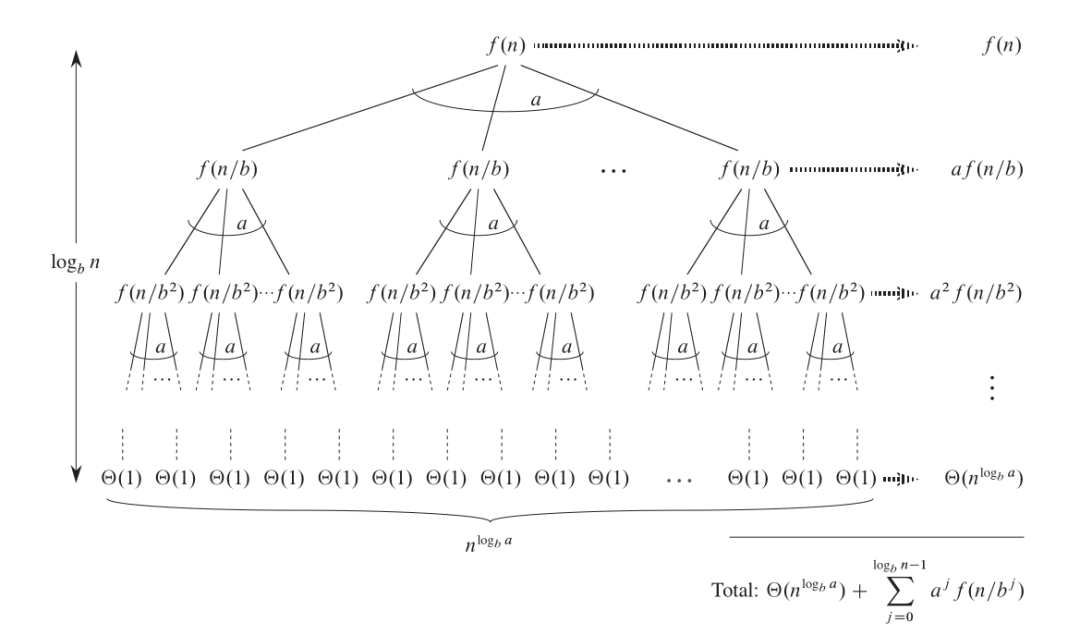
\includegraphics[scale=0.4]{图一.png}
    \caption[图一]{}\label{fig-图一}
\end{figure}

如果将任意一个非叶子节点看作根节点,这都将是一个完整的分治问题的递归树,所以在固定问题中每一层的计算代价不会无规律的变化,复杂度的分布只会有三种情况:\\
1.从树根到叶子每一层来看复杂度越来越高;\\
2.从根节点到叶子节点每层来看复杂度排布均匀;\\
3.从树根到叶子每一层来看复杂度越来越低.


届时我们需要考虑总体递归式的算法时间复杂度将由这两项决定,因为叶子节点已经完全确定了复杂度的渐进紧确界.以上三种情况分别对应:\\
1.整体代价叶子节点决定;\\
2.整体代价均匀分布;\\
3.整体代价根节点决定.


令$g(n)=\sum_{j=0}^{\log_bn-1}a^jf(n/b^j)$
并将其与由叶子节点确定的紧确界进行比较.\\
1.如果$f(n)=O(n^{\log _ba-\epsilon})$,其中$\epsilon$为大于零的常数,那么:
\begin{align*}
g(n)&=O(\sum^{\log_bn-1}_{j=0}a^j(\frac{n}{b^j})^{\log_ba-\epsilon}) \\
    &=O(n^{\log_ba-\epsilon}\sum^{\log_bn-1}_{j=0}a^j(\frac{1}{b^{\log_ba-\epsilon}})^j) \\
    &=O(n^{\log_ba-\epsilon}\sum^{\log_bn-1}_{j=0}(\frac{a}{a*b^{-\epsilon}})^j) \\
    &=O(n^{\log_ba-\epsilon}\sum^{\log_bn-1}_{j=0}b^{\epsilon j})\\
    &=O(n^{\log_ba-\epsilon})(\frac{b^{\epsilon\log_bn}-1}{b^{\epsilon}-1})\\
    &=O(n^{\log_ba-\epsilon}\frac{n^{\epsilon}-1}{b^{\epsilon}-1})\\
    &=O(n^{\log_ba-\epsilon})n^{\epsilon}\\
    &=O(n^{\log_ba}) .\label{eq:cubesum}
\end{align*}
2.如果$f(n)=\Theta(n^{\log _ba})$,那么类似的有:
\begin{align*}
g(n)&=\Theta(\sum_{j=0}^{\log_bn-1}a^j(\frac{n}{b^j})^{\log_ba}) \\
    &=\Theta(n^{\log_ba}\sum^{\log_bn-1}_{j=0}a^j(\frac{1}{b^{\log_ba}})^j) \\
    &=\Theta(n^{\log_ba}\sum^{\log_bn-1}_{j=0}1) \\
    &=\Theta(n^{\log_ba}\log_bn) \\
    &=\Theta(n^{\log_ba}\lg n) .
\end{align*}
3.如果$f(n)=\Omega(n^{\log _ba+\epsilon})$,其中$\epsilon$为大于零的常数,并且当n足够大时存在某个常数$c<1$使得$af(n/b)\le cf(n)$成立,那么:
\begin{align*}
af(\frac{n}{b})&\le cf(n),\\
f(\frac{n}{b})&\le\frac{c}{a}f(n),\\
&\cdots\\
f(\frac{n}{b^j})&\le(\frac{c}{a})^jf(n),\\
a^jf(\frac{n}{b^j})&\le c^jf(n),
\end{align*}
因而:
\begin{align*}
g(n) &=\sum^{\log_bn-1}_{j=0}a^jf(\frac{n}{b^j})\\
     &\le \sum^{\log_bn-1}_{j=0}c^jf(n)\\
     &\le f(n)\sum^{\infty}_{j=0}c^j+O(1)\\
     &\le f(n)\frac{1}{1-c}+O(1)\\
     &=O(f(n)).
\end{align*}
又因为\[g(n) =\Omega(f(n))\]
因此有:\\
1.\begin{align*}
T(n) &=\Theta(n^{\log_ba})+O(n^{\log_ba})\\
     &=\Theta(n^{\log_ba}).
\end{align*}
2.\begin{align*}
T(n) &=\Theta(n^{\log_ba})+\Theta(n^{\log_ba}\lg n)\\
     &=\Theta(n^{\log_ba}\lg n).
\end{align*}
3.\begin{align*}
T(n) &=\Theta(n^{\log_ba})+\Theta(f(n))\\
     &=\Theta(f(n)).
\end{align*}
得证.
\section{定理应用}
\subsection{大整数乘法的分析}
大整数乘法是分治法的具体应用.设X和Y是n位的二进制整数,为求它们的乘积XY,将X和Y分为2段,每段长为$n/2$位(假设n是2的幂).
由此,可将X、Y分别表示为$A2^{n/2}+b,C2^{n/2}+D$,X和Y的乘积为
\begin{align*}
XY &=(A2^{n/2}+B)(C2^{n/2}+D)\\
   &=AC2^n+(AD+BC)2^{n/2}+BD\\
   &=AC2^n+((A-B)(D-C)+AC+BD)2^{n/2}+BD,
\end{align*}
这样只需作3次$n/2$位乘法,因此,
%参考文献里的那个公式
%第二个应用结尾要引用李卿
\begin{equation*}\label{eq:dirichlet}
 T(n)=\begin{cases}
 O(1), &n=1;\\
  3T(n/2)+O(n), &n>1.
  \end{cases}
  \end{equation*}
使用主定理求解,$a=3,b=2$,则
\[n^{\log_ba}=n^{\log_23}=\Theta(n^{1.59}),f(n)=O(n^{\log_23-\varepsilon}),\]
其中$\varepsilon=1$.第一种情况成立,故递归式的解为
\[T(n)=\Theta(n^{\log_ba})=\Theta(n^{1.59}).\]
\subsection{二路并归算法的分析}
并归算法的思路是将两个有序表合并成一个有序表.
对于拥有n个元素的表,其合并表的时间花费为n.\cite{a}因此,二次并归算法的时间复杂度可使用递归式
$T(n)=2T(n/2)+n$表示.
使用主定理求解,$a=2,b=2,f(n)=n$,则
\[n^{\log_ba}=n^{\log_22}=\Theta(n),\]
第二种情况成立,故递归式的解为
\[T(n)=\Theta(n^{\log_ba}\lg n)=\Theta(n\lg n).\]
\subsection{满足第三种情况的案例}
已知递归式$T(n)=3T(n/4)+a\log n$.
使用主定理求解,$a=3,b=4,f(n)=n\log n$,则
\[n^{\log_43}=O(n^{0.793}),f(n)=\Omega(n^{\log_43+\varepsilon}),\varepsilon\thickapprox 0.2,\]
且当$c=0.75,n$充分大时,有
\[af(n/b)=3(n/4)\log (n/4)\le(3/4)n\log n=cf(n),\]
即第三种情况成立,故递归式的解为
\[T(n)=\Theta(n\log n).\]
\nocite{*}
\bibliography{Task2}
\end{document}
